%编译链是txs:///xelatex | txs:///biber | txs:///xelatex | txs:///xelatex | txs:///view

\documentclass{beamer}
\usepackage{ctex, hyperref}
\usepackage{calligra}
\usepackage[]{amsmath}
\usepackage{amssymb}
\usepackage{annotate-equations}
\usepackage{utfsym}
\usepackage[]{adjustbox}
\usepackage{calligra}
\usepackage{extpfeil}
\usepackage[T1]{fontenc}

\usepackage[style=alphabetic]{biblatex}  % 改用biber
\addbibresource{ref.bib}

% 清除冗余字段(期刊、出版社、页码等)
% 这样参考文献列表除了作者年份和论文题目,其它的都不会输出
\AtEveryBibitem{
	\clearlist{language}     % 清除语言字段
	\clearfield{journaltitle} % 期刊名称
	\clearfield{volume}       % 卷号
	\clearfield{number}       % 期号
	\clearfield{pages}        % 页码
	\clearlist{publisher}     % 出版社
	\clearlist{location}      % 出版地
	\clearfield{isbn}         % ISBN
	\clearfield{issn}         % ISSN
	\clearfield{note}         % 备注
	\clearfield{eprint}       % arXiv 号(二次确认)
	\clearfield{doi}
	\ifentrytype{article}{    % 针对期刊文章额外清理
		\clearfield{urldate}     % 访问日期
	}{}
}

%% 作者部分
\author{郑卜凡}
\title{纯旋量超弦}
\subtitle{本科毕业答辩}
\institute{指导老师:杜一剑}
\date{2025年5月11日}
\usepackage{WHU}
% 调整页面左右边距
\setbeamersize{text margin left=0.3cm, text margin right=0.3cm}

\setlength{\parindent}{0pt} % 取消所有段落缩进
%自定义命令
%% 实现双重尖括号
\makeatletter
\newsavebox{\@brx}
\newcommand{\llangle}[1][]{\savebox{\@brx}{\(\m@th{#1\langle}\)}%
	\mathopen{\copy\@brx\kern-0.5\wd\@brx\usebox{\@brx}}}
\newcommand{\rrangle}[1][]{\savebox{\@brx}{\(\m@th{#1\rangle}\)}%
	\mathclose{\copy\@brx\kern-0.5\wd\@brx\usebox{\@brx}}}
\makeatother

\begin{document}

\kaishu
\begin{frame}
	\titlepage
	\begin{figure}[htpb]
		\begin{center}
			
\includegraphics[width=0.2\linewidth]{pic/whulogo.eps}
		\end{center}
	\end{figure}
\end{frame}
\begin{frame}
\tableofcontents[sectionstyle=show,subsectionstyle=show/shaded/hide,subsubsectionstyle=show/shaded/hide]
\end{frame}


\section{为什么要研究弦振幅?}

\begin{frame}{为何在能标远低于Planck能标情况下还要研究弦振幅?}
\begin{itemize}
\item {\color{WHU} 历史起源说:}\\
	弦理论第一个公式是Veneziano公式,提出时是作为强相互作用的经验公式,后来发现实则是四快子开弦振幅
\item {\color{WHU} 场论学家说:}\\
	弦理论在弦长极限下退化为量子场论,所以对弦振幅的研究有助于理解场论振幅,比如KLT关系\cite{Kawai:1985xq}给出规范理论振幅和引力振幅的内在联系;世界面积分的想法催生了量子场论振幅的CHY公式\cite{Cachazo:2013iea,Cachazo:2013hca}
\item {\color{WHU} 数学家也说}:\\
	弦理论的发展涉及到许多前沿数学的应用,近年研究指出弦理论振幅可以看作是数论函数,如Multi Zeta Values,的生成函数,从而与数学产生联系\cite{Broedel:2013aza}
\end{itemize}
\end{frame}

\section{纯旋量超弦}

\begin{frame}{RNS超弦不香吗?}
	由于玻色弦存在不稳定真空以及无法描述费米子等问题,通过加入超对称便可得到费米子自由度,最早发展的一类超弦是通过添加世界面旋量得到的{\color{WHU} RNS超弦}:
	\only<1>{\begin{equation}
		S=\frac{1}{2\pi}\int\mathrm{d}^{2}z\left(\frac{2}{\alpha^{\prime}}\partial X^{\mu}\overline{\partial}X_{\mu}+\psi^{\mu}\overline{\partial}\psi_{\mu}+\overline{\psi}^{\mu}\partial\overline{\psi}_{\mu}\right)
	\end{equation}}
	\only<2>{\begin{equation*}\tag{1}
		\tikzmarknode{node}{S=\frac{1}{2\pi}\int\mathrm{d}^{2}z\left(\frac{2}{\alpha^{\prime}}\partial X^{\mu}\overline{\partial}X_{\mu}+\psi^{\mu}\overline{\partial}\psi_{\mu}+\overline{\psi}^{\mu}\partial\overline{\psi}_{\mu}\right)}
	\end{equation*}
	\annotate[yshift=0.6em]{}{node}{{\color{WHU}Hide} target spacetime SUSY}}
	
	% 这里讲振幅是靶空间超对称的量,所以在振幅计算上RNS超弦复杂一些
	再利用一圈配分函数模不变性要求的{\color{WHU} GSO投影}便可以剔除快子态并且匹配玻色和费米自由度。但是真正需要的靶空间超对称在RNS超弦中被隐藏。后续又发展了靶空间超对称的{\color{WHU} GS超弦}:
	\only<1>{\begin{equation}
		S_{\mathrm{GS}}=\frac{1}{\pi}\int d^{2}z\left[\frac{1}{2}\Pi^{m}\overline{\Pi}_{m}+\frac{1}{4}\Pi_{m}(\theta\gamma^{m}\overline{\partial}\theta)-\frac{1}{4}\overline{\Pi}_{m}(\theta\gamma^{m}\partial\theta)\right]
	\end{equation}}
	\only<2>{\begin{equation}\tag{2}
			S_{\mathrm{GS}}=\frac{1}{\pi}\int d^{2}z\tikzmarknode{node}{\left[\frac{1}{2}\Pi^{m}\overline{\Pi}_{m}+\frac{1}{4}\Pi_{m}(\theta\gamma^{m}\overline{\partial}\theta)-\frac{1}{4}\overline{\Pi}_{m}(\theta\gamma^{m}\partial\theta)\right]
		}
	\end{equation}
	\annotate[yshift=0em]{below}{node}{{\color{WHU}Break} Lorentz covariant }}
	
	但是其只能在光锥坐标下量子化!
\end{frame}

\begin{frame}{鱼与熊掌不可兼得}
这两种方案都不完美,振幅计算上RNS超弦拥有洛伦兹协变的顶角算符从而更加方便,但对于非平凡靶空间背景下超弦理论的构造GS形式有更多优势。Siegle后续又对GS形式进行了改进使得其可以协变量子化:
\begin{equation}
	S_{\mathrm{Siegel}}=\frac{1}{\pi}\int d^2z\left[\frac{1}{2}\partial X^m\overline{\partial}X_m+p_\alpha\overline{\partial}\theta^\alpha\right]
\end{equation}
但是这一方案与RNS超弦不等价,关键在于RNS超弦和Siegle超弦都有非平凡的洛伦兹Noether流\only<2>{,但它们的算符乘积展开不同}:
\only<1>{
\begin{equation*}
	\Sigma_{\mathrm{RNS}}^{mn}=-\psi^m\psi^n,\quad\Sigma_{\mathrm{Siegel}}^{mn}=-\frac{1}{2}(p\gamma^{mn}\theta)
\end{equation*}
}
\onslide<2>{\begin{equation*}
	\Sigma_{\mathrm{RNS}}^{mn}(z)\Sigma_{\mathrm{RNS}}^{pq}(w)\sim\frac{\delta^{p[m}\Sigma^{n]q}(w)-\delta^{q[m}\Sigma^{n]p}(w)}{z-w}+\frac{\delta^{m[q}\delta^{p]n}}{(z-w)^2}
\end{equation*}}
\onslide<2>{\begin{equation*}
	\Sigma_{\mathrm{Siegel}}^{mn}(z)\Sigma_{\mathrm{Siegel}}^{pq}(w)\sim\frac{\delta^{p[ m}\Sigma^{n] q}(w)-\delta^{q[ m}\Sigma^{n] p}(w)}{z-w}+{\color{red} 4}\frac{\delta^{m[ q}\delta^{p] n}}{(z-w)^2}
\end{equation*}}
\end{frame}


\begin{frame}{Berkovits的天才想法}
	Berkovits试图通过在Siegle形式中加入一对玻色鬼场$(\lambda_\alpha, w^\alpha)$,从而将Sigle超弦的Lorentz流补充为$\Sigma^{mn}+N^{mn}$,不难发现只要有下面OPE成立就有希望得到Lorentz协变、靶空间超对称且等价于RNS超弦的形式:
	\begin{equation}
		\label{eq:2}
		N^{mn}(z)N^{pq}(w)\sim\frac{\delta^{p[m}N^{n]q}(w)-\delta^{q[m}N^{n]p}(w)}{z-w}-3\frac{\delta^{m[q}\delta^{p]n}}{(z-w)^2}
	\end{equation}
	Berkovits 通过$U(5)$分解进行计算做到了这一点:\cite{Berkovits:2000fe}
	\begin{equation}\label{eq:3}
		S_{\mathrm{PS}}=\frac{1}{\pi}\int d^2z\left(\frac{1}{2}\partial X^m\overline{\partial}X_m+p_\alpha\overline{\partial}\theta^\alpha-w_\alpha\overline{\partial}\lambda^\alpha\right)
	\end{equation}\only<1>{BRST算符幂零,$Q_{\mathrm{BRST}}^2=0$,要求靶空间旋量满足约束$\lambda \gamma^\mu \lambda = 0$,数学上称$\lambda_\alpha$为{\color{WHU}纯旋量}。所以Berkovits发现的这以理论形式也被称为{\color{WHU}纯旋量超弦}。}\only<2>{由于纯旋量约束所以(\ref{eq:3})不是自由CFT,但是Berkovits将其$U(5)$分解到自由变量后发现刚好会给出正确的OPE补偿(\ref{eq:2})。而且中心荷$c_{\text{Siegle}}=-22\neq 0$,$\lambda w$鬼场刚好补偿了这一中心荷。}
\end{frame}


\section{盘面散射振幅}
\begin{frame}
不同于场振幅按照顶点个数展开,弦论振幅微扰展开是由世界面欧拉数决定的:
\begin{figure}[htpb]
	\centering
	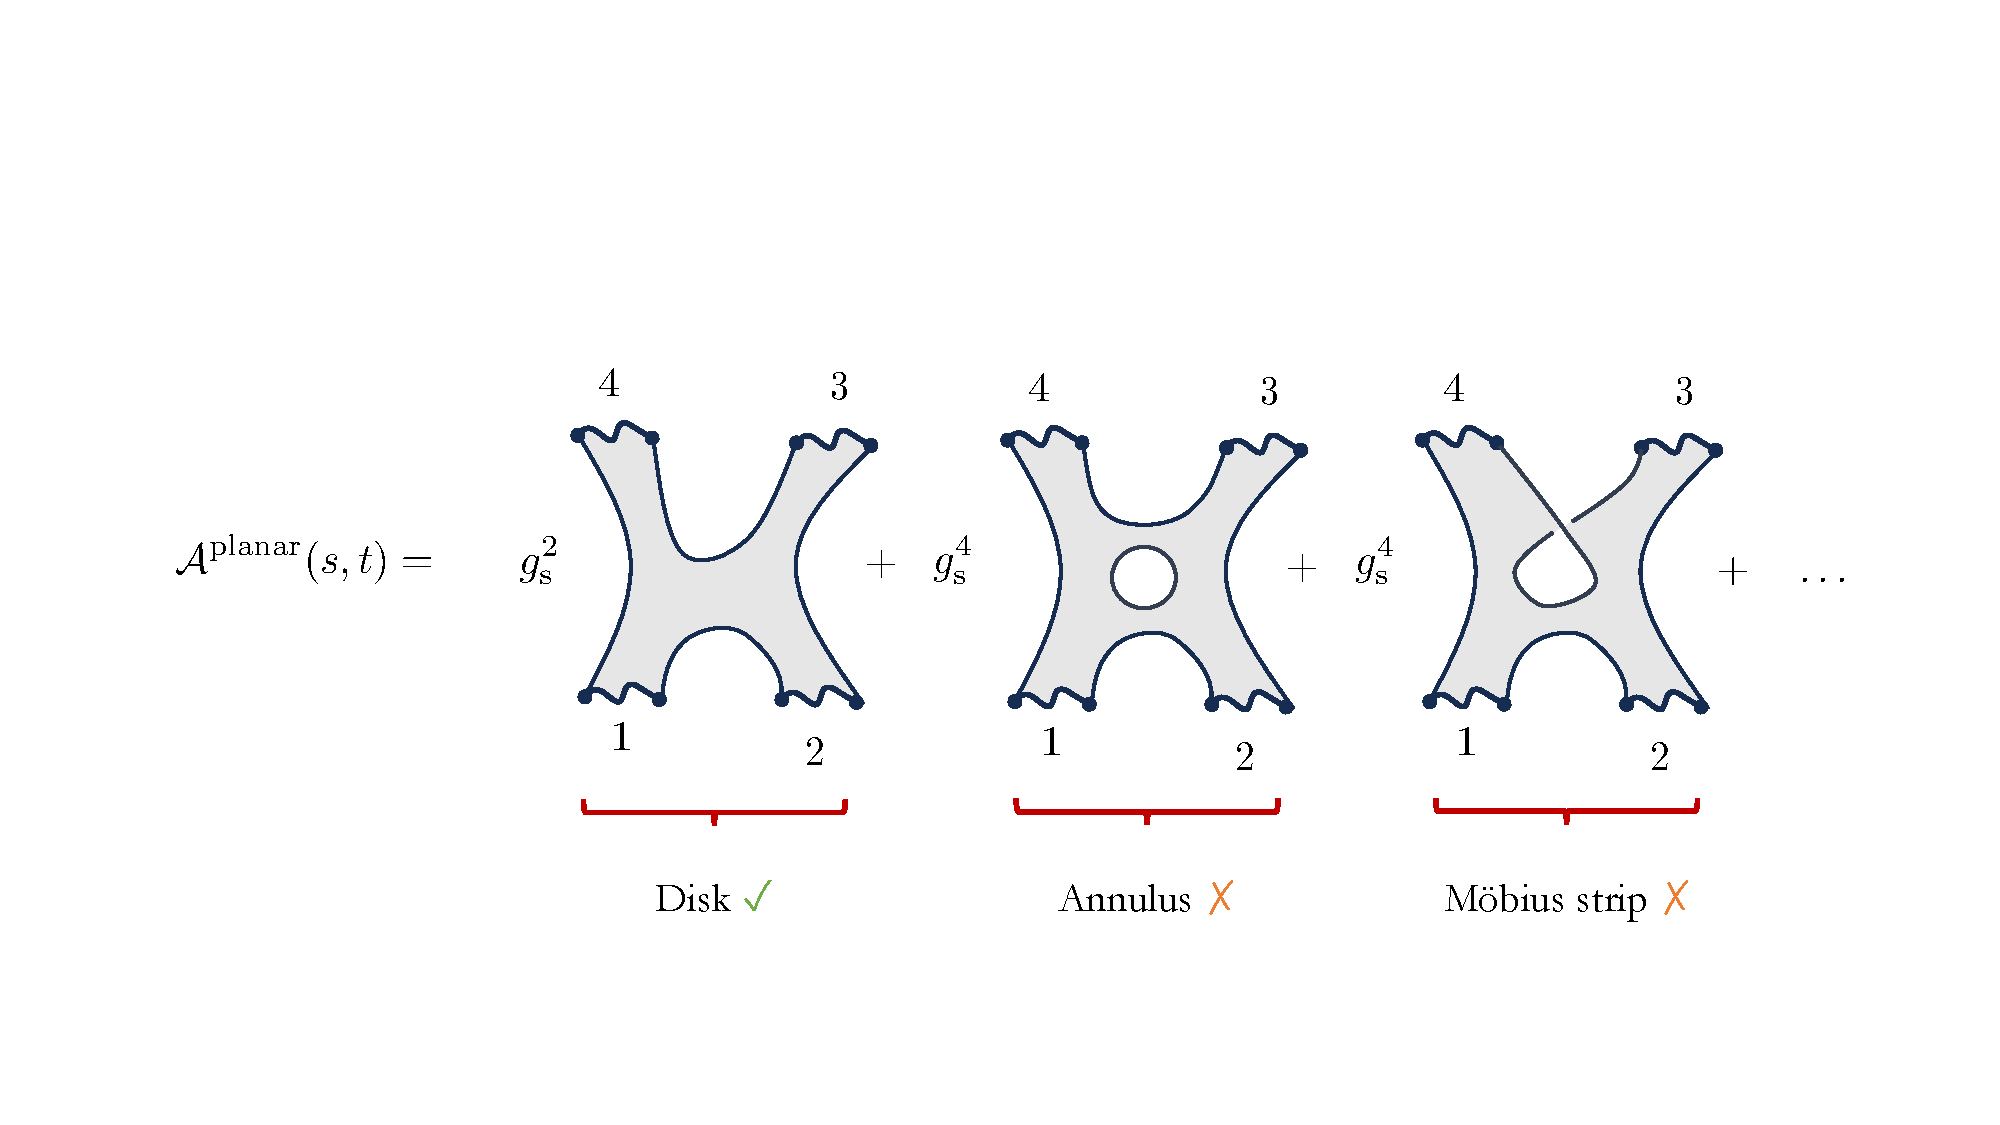
\includegraphics[width=\linewidth]{pic/1.pdf}
\end{figure}

后面关注开弦振幅最低阶,{\color{WHU}盘面振幅}的贡献。纯旋量超弦一般的盘面振幅由下面的公式给出:
\begin{equation}\label{eq:4}
	\mathcal{A}(P)=\int_{D(P)}dz\llangle V_1(z_1)U_2(z_2)\ldots U_{n-2}(z_{n-2})V_{n-1}(z_{n-1})V_n(z_n)\rrangle
\end{equation}
\end{frame}

\begin{frame}
BRST量子化得到的无质量态积分顶角算符$U$和无积分顶角算符$V$为:
\begin{equation*}
\begin{aligned}
		U(z)&=\partial\theta^\alpha A_\alpha(X,\theta)+A_m(X,\theta)\Pi^m+d_\alpha W^\alpha(X,\theta)+\frac{1}{2}N_{mn}F^{mn}(X,\theta)\\
	V(z)&=\lambda^\alpha A_\alpha(X,\theta),\quad \{A_{\alpha/m},W^\alpha,F^{mn}\}\,(\text{a.k.a. } K)\in 10\text{D SYM}
\end{aligned}
\end{equation*}

\only<1>{(\ref{eq:4})中关联函数计算第一步是利用物质场OPE展开顶角算符OPE:
\begin{equation*}
	\begin{gathered}
		X^\mu(z,\overline{z}) X^\nu(w,\overline{w}) 
		\sim -\eta^{\mu\nu} \ln|z-w|^2, \quad
		 d_\alpha(z) \theta^\beta(w) 
		\sim \frac{\delta_\alpha^\beta}{z-w}, \\
		d_\alpha(z) d_\beta(w) 
		\sim -\frac{\gamma_{\alpha\beta}^\mu \Pi_\mu(w)}{z-w}, \quad 
		 d_\alpha(z) \Pi^\mu(w) 
		\sim \frac{(\gamma^\mu \partial\theta(w))_\alpha}{z-w}, \\
		\Pi^\mu(z) \Pi^\nu(w) 
		\sim -\frac{\eta^{\mu\nu}}{(z-w)^2}, \quad
		d_\alpha(z)K\sim\frac{D_\alpha K}{z-w},
		\quad\Pi^m(z)K\sim-\frac{\partial^mK}{z-w}
	\end{gathered}
\end{equation*}
\begin{equation*}
\begin{gathered}
		D_\alpha=\frac{\partial}{\partial\theta^\alpha}+\frac{1}{2}(\gamma^\mu\theta)_\alpha\partial_\mu,\quad \Pi^m=\partial X^m+\frac{1}{2}(\theta\gamma^m\partial\theta)\\
	d_\alpha=p_\alpha-\frac{1}{2}{\left(\partial X^m+\frac{1}{4}(\theta\gamma^m\partial\theta)\right)}(\gamma_m\theta)_\alpha
\end{gathered}
\end{equation*}
}

\only<2>{第二步是把超场按照$\theta$展开,这个时候$K$关于$X$的平面波依赖已经被物质场OPE吸收了,只剩下鬼场零模需要计算,它们与世界面坐标无关,鬼场积分测度为:
	\begin{equation}
		\left\langle(\lambda\gamma^m\theta)(\lambda\gamma^n\theta)(\lambda\gamma^p\theta)(\theta\gamma_{mnp}\theta)\right\rangle=2880 
	\end{equation}
}
而SYM超场的展开式十分复杂,比如:
\begin{equation}
	A_i^m(X,\theta)=\left\{(\cosh\sqrt{O})^m{}_qe_i^q+\left(\frac{\sinh\sqrt{O}}{\sqrt{O}}\right)^m{}_q(\theta\gamma^q\chi_i)\right\}\mathrm{e}^{k\cdot X}
\end{equation}
其中选取了$i k^\mu\to k^\mu$的符号约定,$O^m{}_q:=\frac{1}{2}(\theta\gamma^m{}_{qn}\theta)k_i^n$.
\end{frame}

\begin{frame}
	纯旋量超弦虽然在描述圈级振幅上相较于RNS超弦更有利,但是树级振幅计算乍看起来优势并不明显。但是倘若我们将顶角算符看作一个整体,他们的OPE之间有非常神奇的规律,且具有{\color{WHU}自由李代数结构}:
	\begin{equation}
		V_A(z_a)U_B(z_b)\sim\frac{V_{[A,B]}(z_b)}{z_{ab}},\quad U_A(z_a)U_B(z_b)\sim\frac{U_{[A,B]}(z_b)}{z_{ab}}
	\end{equation}
	这里指标$A$可以是一个李多项式,而不必是单粒子指标,其定义只需要做指标替换$K_i\to K_A$,而{\color{WHU}多粒子超场}$K_A$和单粒子超场$K_i$之间又存在{\color{WHU}确定的}递推关系\only<1>{,比如Lorenz规范下:
	{\small
	\begin{equation*}
		\begin{aligned}\hat{A}_{\alpha}^{[P,Q]}&=\frac{1}{2}\left[\hat{A}_{\alpha}^{Q}(k_{Q}\cdot\hat{A}_{P})+\hat{A}Q^{m}(\gamma_{m}\hat{W}_{P})\alpha-(P\leftrightarrow Q)\right]\\\hat{A}_{[P,Q]}^{m}&=\frac{1}{2}\left[\hat{A}_{Q}^{m}(k_{Q}\cdot\hat{A}_{P})+\hat{A}_{n}^{P}\hat{F}_{Q}^{nm}+(\hat{W}_{P}\gamma^{m}\hat{W}_{Q})-(P\leftrightarrow Q)\right]\\\hat{W}_{[P,Q]}^{\alpha}&=\frac{1}{4}\hat{F}_{P}^{rs}(\gamma_{rs}\hat{W}_{Q})^{\alpha}+\frac{1}{2}(k_{Q}\cdot\hat{A}_{P})\hat{W}_{Q}^{\alpha}+\frac{1}{2}\hat{W}_{Q}^{m\alpha}\hat{A}_{m}^{P}-(P\leftrightarrow Q)\\\hat{F}_{[P,Q]}^{mn}&=\frac{1}{2}\left[\hat{F}_{Q}^{mn}(k_{Q}\cdot\hat{A}_{P})+\hat{F}_{Q}^{p|mn}\hat{A}_{p}^{p}+\hat{F}_{Q}^{[m}\hat{F}_{P}^{n]r}-2\gamma_{\alpha\beta}^{[m}\hat{W}_{P}^{n]\alpha}\hat{W}_{Q}^{\beta}-(P\leftrightarrow Q)\right]
		\end{aligned}
	\end{equation*}}
	}
	
	% 用only会导致编号出现问题,使用类似的命令\uncover则不会
	\uncover<2>{
	所以其实可以递推地得到任意点无质量态盘面振幅:\cite{Mafra:2011nv,Mafra:2011nw}
	{\footnotesize
	\begin{equation}
		\label{eq:8}
		\boxed{\mathcal{A}_{n}(P)=(2\alpha^{\prime})^{n-3}\int d\mu_{P}^{n}\sum_{AB=23...n-2}\langle(V_{1A}\mathcal{Z}_{1A})(V_{(n-1)\tilde{B}}\mathcal{Z}_{n-1,\tilde{B}})V_{n}\rangle+\mathrm{perm}}
	\end{equation}}
	{\footnotesize
	\begin{equation*}
		\mathcal{Z}_{123\cdots p}:=\frac{1}{z_{12}z_{23}\cdots z_{p-1,p}},\quad \int d\mu_P^n:=\int_{D(P)}dz_2dz_3\cdots dz_{n-2}\prod_{1\leq i<j}^{n-1}|z_{ij}|^{-2\alpha^{\prime}s_{ij}}
	\end{equation*}}
	}
\end{frame}

\section{构建SYM树图BCJ分子}
\begin{frame}{色-运动学对偶}
	考虑将规范理论用三顶角图(不必是费曼图)编码:
	\begin{equation}\label{eq:9}
		\mathcal{A}_n=\sum_{i\in\Gamma_n}\frac{c_iN_i}{D_i}
		\only<2>{\color{blue} \xRightarrow[\text{Loop }\exists \{N_i\}  ?]{\text{Tree }\exists \{N_i\}  \checkmark}\mathcal{M}_n=\sum_{i\in\Gamma_n}\frac{N_iN_i}{D_i}=\sum_{i\in\Gamma_n}\frac{N_i\tilde{N}_i}{D_i}}
	\end{equation}
	这里极点$D_i$完全由内线给出,并不是重点. 分子部分\cite{Bern:2008qj}猜想存在一种编码方式,使得$\{N_i\}$满足和色因子$\{c_i\}$由图的顶点结构给出的相同的Lie代数结构:
	\begin{figure}[htpb]
		\centering
		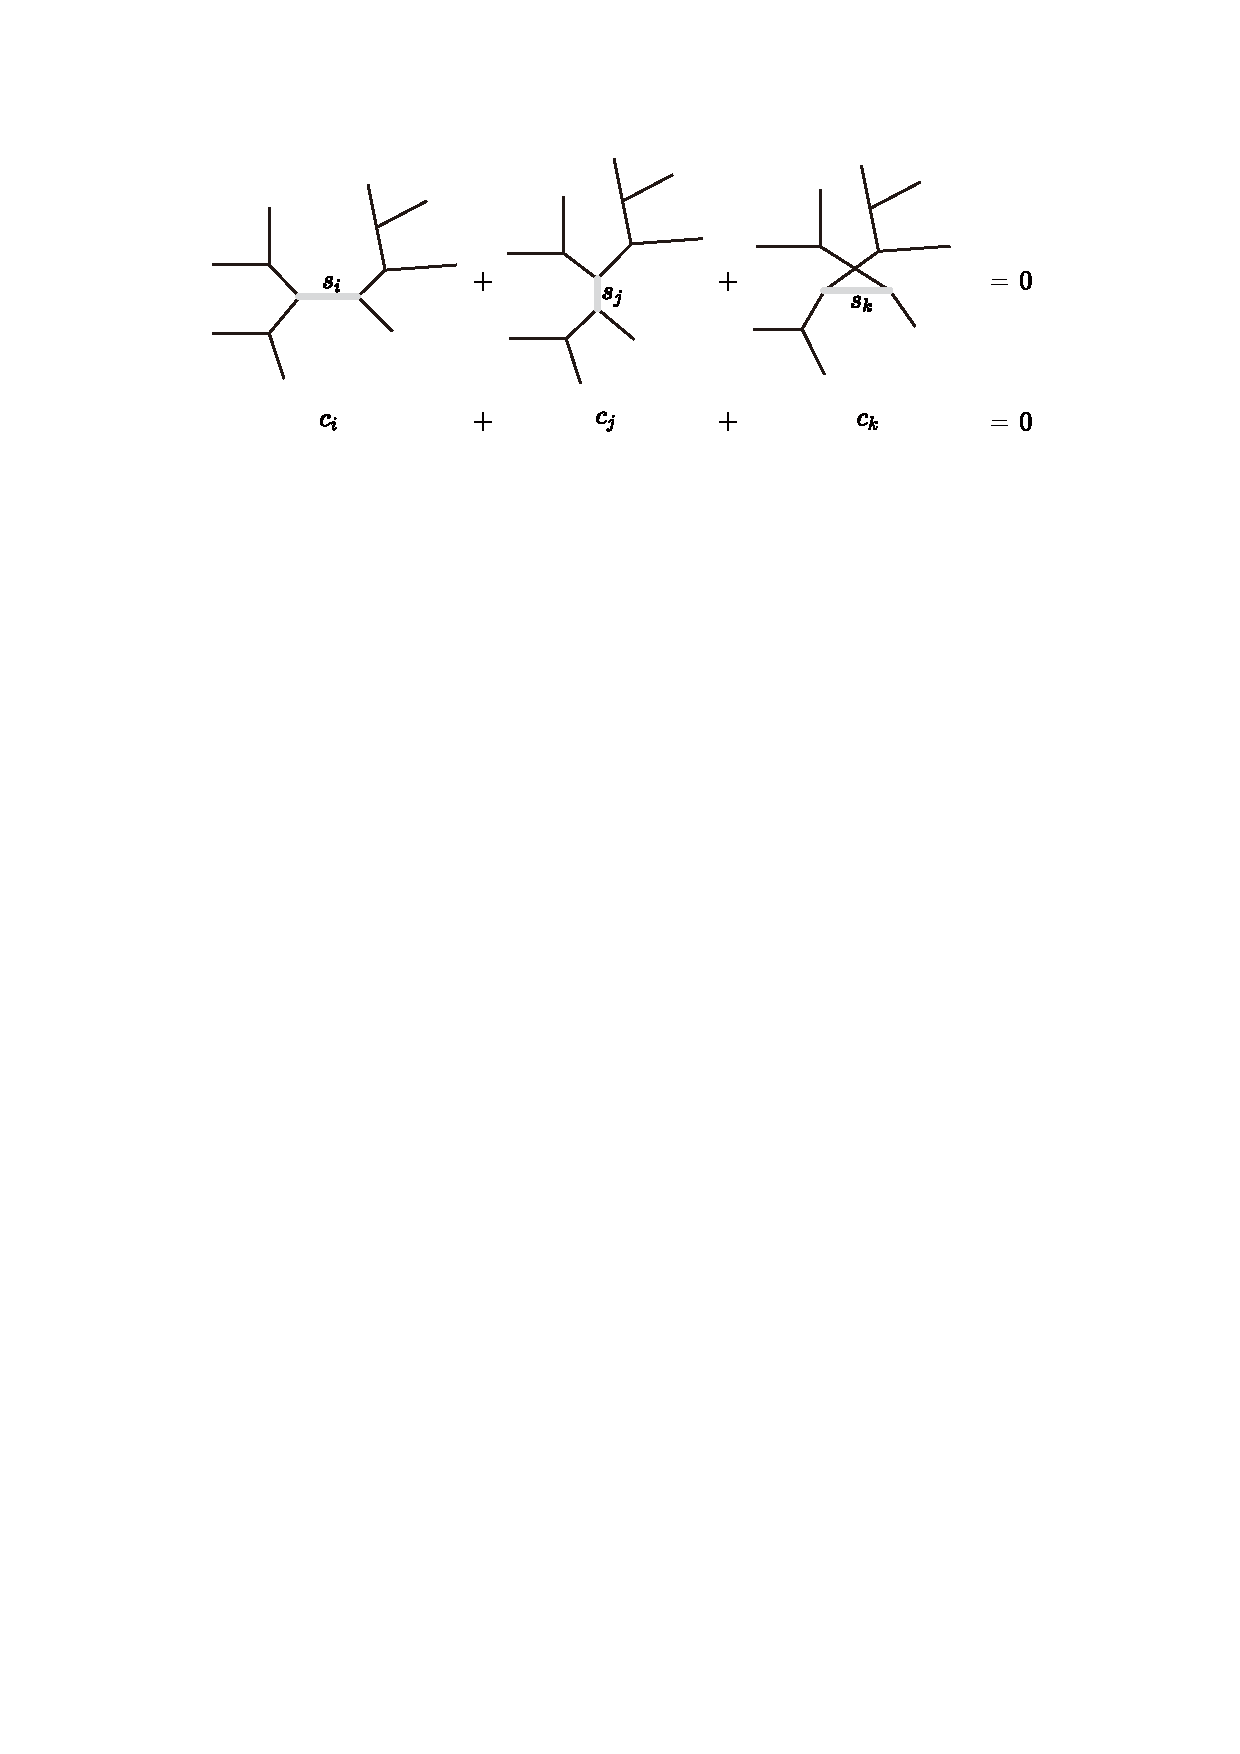
\includegraphics[width=0.60\linewidth]{pic/2.pdf}
	\end{figure}
	而一旦得到这样的$\{N_i\}$,只用将$\{c_i\}$也替换为$\{N_i\}$便可得到微扰引力振幅!这样的分子称为{\color{WHU} BCJ分子}。
\end{frame}

\begin{frame}
	\only<1>{在DDM基底下可以将(\ref{eq:9})写成下面的形式:\cite{DelDuca:1999rs}
	\begin{equation*}
		\mathcal{A}_n^\mathrm{gauge}=\sum_{P,Q\in S_{n-2}}c_{1|P|n}m(1,P,n|1,Q,n)N_{1|Q|n}\quad m(\bullet|\bullet) \text{ for }\operatorname{tr}\phi^3 \text{ Amp.}
	\end{equation*}}
	\only<2->{{\color{red}仍在DDM基底下展开,但写成偏振幅形式且对外腿进行适当重排:
		\begin{equation*}
		\mathcal{A}_n(P)^\mathrm{gauge}=\sum_{Q\in S_{n-2}}N_{1|Q|n-1}m(P|1,Q,n-1),\quad \sum_Q \sim \sum_{AnB}+\mathrm{perm}
	\end{equation*}}}
	这些$\{N_i\}$之间相互独立,所以只要我们将SYM振幅写成上面的形式,就能立即读出BCJ分子,而纯旋量超弦很容易做到这一点\cite{Mafra:2011kj}。首先利用$Z$积分可以将超弦振幅(\ref{eq:8})改写为:
	\only<1>{{\footnotesize
	\begin{equation}
		\boxed{\mathcal{A}_n(P)=\sum_{AB=23\cdots n-2}\langle V_{1A}V_{(n-1)\tilde{B}}V_n\rangle(-1)^{|B|-1}Z(P|1,A,n,B,n-1)+\mathrm{perm}}
	\end{equation}
	}}
	\only<2->{{\footnotesize
		\begin{equation*}
			\color{blue}
			\mathcal{A}_n(P)^\text{string}\xrightarrow{\alpha'\to 0 }\sum_{AB=23\cdots n-2}\langle V_{1A}V_{(n-1)\tilde{B}}V_n\rangle(-1)^{|B|-1}m(P|1,A,n,B,n-1)+\mathrm{perm}
		\end{equation*}
	}}
	{\footnotesize
		\begin{equation}
			Z(P|Q):=(2\alpha^{\prime})^{n-3}\int_{D(P)}\frac{dz_1dz_2\cdots dz_n}{\mathrm{vol}(\mathrm{SL}_2(\mathbb{R}))}\prod_{i<j}^n|z_{ij}|^{-2\alpha^{\prime}s_{ij}}\mathrm{PT}(Q)
		\end{equation}
	}
	在弦长极限下$\lim_{\alpha^{\prime}\to0}Z(P|Q)=m(P|Q)$,$\mathcal{A}_n(P)^\text{string}\to\mathcal{A}_n(P)^{\text{gauge}}$
	\onslide<3>{\[\Rightarrow \boxed{N_{1|AnB|n-1}=(-1)^{|B|-1}\langle V_{1A}V_{(n-1)\tilde{B}}V_n\rangle}\]
	这样便显式地构造出了BCJ分子!\hfill$\square$}
\end{frame}

% ==== 独立致谢帧 ====
\section*{特别鸣谢}  % 无编号节(不显示在目录/导航栏)
\addtocontents{toc}{\protect\setcounter{tocdepth}{-5}}  % 阻止写入目录

\begin{frame}
	\begin{center}
		{\Huge Thanks!}
	\end{center}
	\vspace{0.3cm}
	\begin{columns}[b] % [T] 顶部对齐
		% 左栏照片 + 署名
		\begin{column}{0.48\textwidth} % 留出间距
			\centering
			\adjustbox{width=\linewidth, height=3cm, keepaspectratio, margin=0pt}{
\includegraphics[width=0.9\linewidth]{pic/huang.jpg}}% 调整图片宽度
			\\
			\vspace{0.1cm} % 图片与署名间距
			\textbf{\color{WHU}Yu-tin Huang}  % 署名(颜色匹配模板主题)
		\end{column}
		
		% 右栏照片 + 署名
		\begin{column}{0.48\textwidth}
			\centering
			\adjustbox{width=\linewidth, height=3cm, keepaspectratio, margin=0pt}{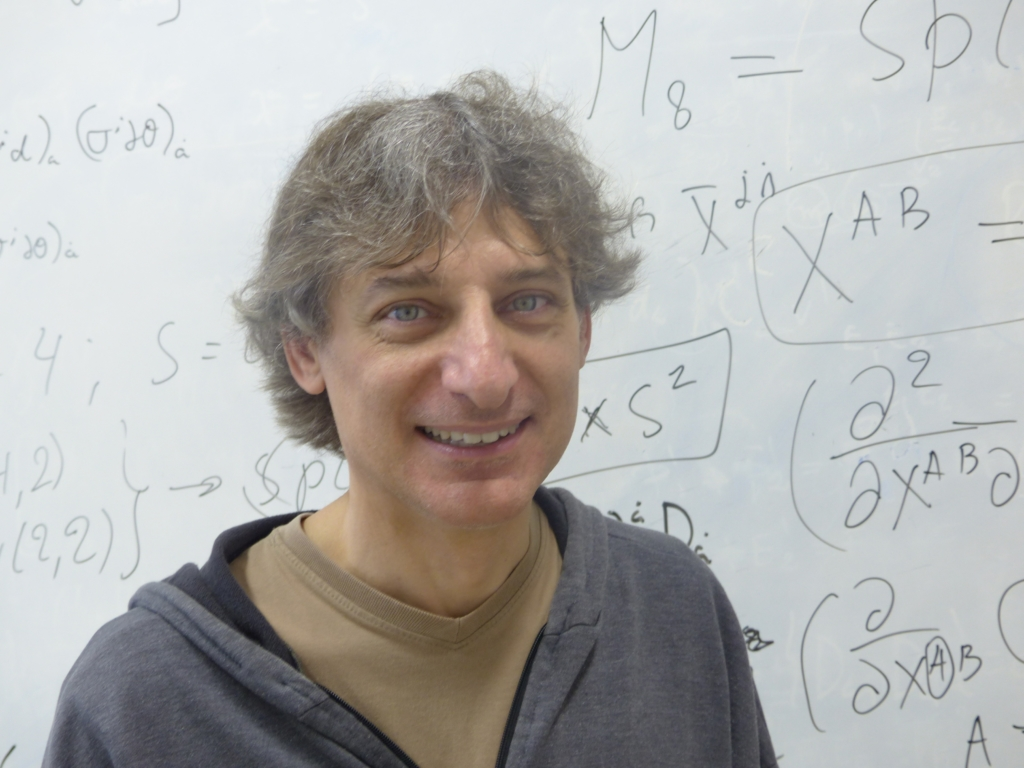
\includegraphics[width=0.9\linewidth]{pic/berkovits.jpg}}
			\\
			\vspace{0.1cm}
			\textbf{\color{WHU}Nathan Berkovits}
		\end{column}
	\end{columns}
	
	\begin{center}
		{\Large} {\calligra Your Praise, My Phoenix Flame}
	\end{center}
\end{frame}

% ==== 参考文献列表 ====
\begin{frame}[allowframebreaks]
\printbibliography
\end{frame}

\end{document}